\section{Fundamentação teórica}

\begin{frame}{Sistema de arquivos distribuído}
	
	\begin{columns}
		\column{0.6\textwidth}
		
		\begin{itemize}
			\item Características:
			
			\begin{itemize}
				\item Voltado para gerenciamento e armazenamento de arquivos em larga escala.
				\item Conjunto de vários computadores distribuídos fisicamente, conectados através de rede, se mostrando como se fosse apenas um computador.
				%\item Cria algumas copias de segurança dos dados, chamadas de réplicas, cujas são armazenadas espalhadamente entre os servidores.
				%\item 	
			\end{itemize}
		\end{itemize}
		
		\column{0.4\textwidth}
		
		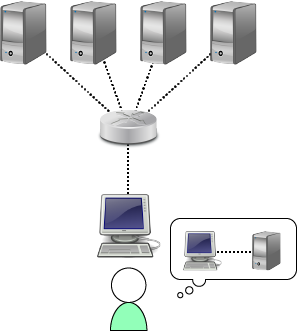
\includegraphics[width=\textwidth]{imagens/sad}
	\end{columns}
\end{frame}
	
\begin{frame}{}
	\begin{itemize}
	\item Vantagem e desvantagem:
	\\
	\begin{block}{Vantagem}
		
	Possui maior facilidade e menor custo para aumentar a escala do sistema.
	\end{block}
	\begin{block}{Desvantagem}
	
	Aumento da probabilidade de falhas nos arquivos causado pela aumento dos componentes envolvidos.
	
	\end{block}
	
	\end{itemize}
\end{frame}


\begin{frame}{}
	
	\begin{itemize}
	\item Solução:
	\\
	
		\begin{itemize}
		\item Atribuição de partes redundante nos arquivos para tolerar as possíveis falhas.
		
		
		\item Criação de algumas cópias de segurança dos arquivos, chamadas de réplicas.
		
		\end{itemize}
	\end{itemize}
	
	\begin{center}
		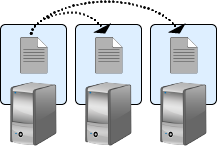
\includegraphics[width=0.5\textwidth]{imagens/replica}
		
	\end{center}
	
\end{frame}
	
\begin{frame}{}
	\begin{itemize}
	\item Consequência:
		
	\begin{itemize}
	\item Replicação de arquivos consegue tolerar as falhas, mas acaba necessitando de espaço extra para armazenar as partes redundantes.

	\item Quando cria duas réplicas, a capacidade total de armazenamento requerida triplica. 

	\end{itemize}
	
	%\item A solução para esta consequência é tentar diminuir o tamanho da parte redundante, utilizando um esquema diferente da replicação. 

	\end{itemize}
\end{frame}


\begin{frame}{}
	\begin{itemize}
	\item Outra característica:
	
	\begin{itemize}
		\item Divisão de papel no gerenciamento de arquivos.
		
		\item Divide os arquivos em duas partes: metadado e dado.

	\end{itemize}
	\end{itemize}
	\begin{center}
	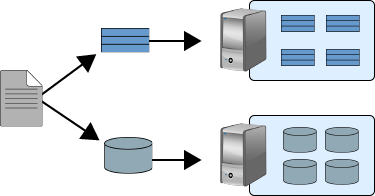
\includegraphics[width=0.6\textwidth]{imagens/meta}
	\end{center}
\end{frame}


\begin{frame}{}
	Metadados
	\\
	
	\begin{tabular}{|l|l|} \hline
		\textbf{Informação} & \textbf{Descrição}  \\ \hline
		name			& Nome do arquivo/diretório \\ \hline
		parent			& Diretório contido \\ \hline
		creationTime	& Tempo de criação \\ \hline
		lastAccessTime	& Tempo de último acesso \\ \hline
		lastModifiedTime& Tempo de última modificação \\ \hline
		size			& Tamanho do arquivo \\ \hline
		lock			& Estado de bloqueio \\ \hline
		
	\end{tabular}
	
	
\end{frame}

\begin{frame}{BFT-SMaRt}
	\begin{itemize}
		\item Biblioteca Java \textit{open-source}.
		\item Características:
		\begin{itemize}
			\item Replicação de máquina de estado (\textit{State Machine
				Replication - }SMR).
			\item Tolerante a falhas bizantinas (\textit{Byzantine Fault-Tolerant - BFT}).
			\item Simplicidade.
			\item Modularidade.
			\item API Simples e Extensível.
			\item Consciência de ambiente Multi-Core.	
			\item Reconfiguração.
		\end{itemize}
	\end{itemize}
\end{frame}

\begin{frame}{BFT-SMaRt}
	\begin{itemize}
		\item Para \textbf{n} réplicas e \textbf{f} falhas
		\begin{itemize}
			\item n $\geq$ 3f+1
			\begin{itemize}
				\item Falhas Bizantinas
			\end{itemize}
			\item n $\geq$ 2f+1
			\begin{itemize}
				\item Falhas de sistema
			\end{itemize}
		\end{itemize}
		
		\item Principais métodos
		\begin{itemize}
			\item appExecuteOdered.	
			\item appExecuteUnodered.
			\item invokeOdered.
			\item invokeUnodered.
		\end{itemize}
		
	\end{itemize}
\end{frame}



\begin{frame}{RAID}
	
	\begin{itemize}
		\item \textit{Redundant Array of Independent Disks}.
		\item Trata-se, basicamente, de uma solução computacional que combina vários discos rígidos (HDs) para formar uma única unidade lógica de armazenamento de dados.
	\end{itemize}
\end{frame}

\begin{frame}{RAID}
	
	\begin{itemize}
		\item Vantagens:
		\begin{itemize}
			\item Dependendo do nível, há maior tolerância a falhas graças a redundância.
			\item O acesso à informação pode se tornar mais rápido, pois os dados são distribuídos a todos os discos.
			\item É possível aumentar a capacidade de armazenamento a qualquer momento com a adição de mais HDs.
		\end{itemize}
	\end{itemize}
\end{frame}

\begin{frame}{RAID}
	\begin{itemize}
		\item Níveis de RAID
		\begin{itemize}
			\item RAID 0
			\item RAID 1
			\item RAID 5
		\end{itemize}
	\end{itemize}
\end{frame}

\begin{frame}{RAID 0}
	\begin{columns}
		\column{0.5\textwidth}
		\begin{itemize}
			\item Striping (fracionamento).
			\item Não oferece proteção contra falhas, pois não existe redundância.
			\item Focado no desempenho. Visto que quanto mais discos houver no sistema, maior é a sua taxa de transferência devido ao paralelismo nas operações de leitura e escrita.
		\end{itemize}
		
		\column{0.25\textwidth}
		\begin{figure}
			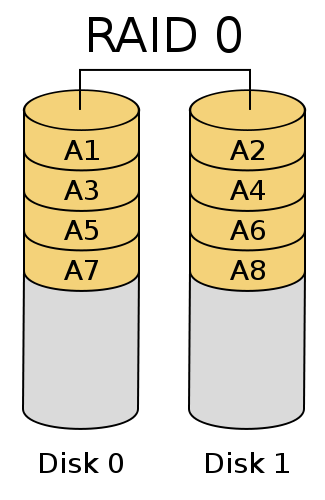
\includegraphics[width=\textwidth]{imagens/RAID_0}
			\label{fig:exemplo}
		\end{figure}
		
	\end{columns}
\end{frame}

\begin{frame}{RAID 1}
	\begin{columns}
		\column{0.5\textwidth}
		\begin{itemize}
			\item Mirror (Espelhamento).
			\item Vantagens
			\begin{itemize}
				\item Evita falhas físicas.
				\item Alto desempenho de leitura.
			\end{itemize}
			\item Desvantagens
			\begin{itemize}
				\item Perda de desempenho de escrita.
				\item Alto desperdício de espaço.
			\end{itemize}
		\end{itemize}
		
		\column{0.25\textwidth}
		\begin{figure}
			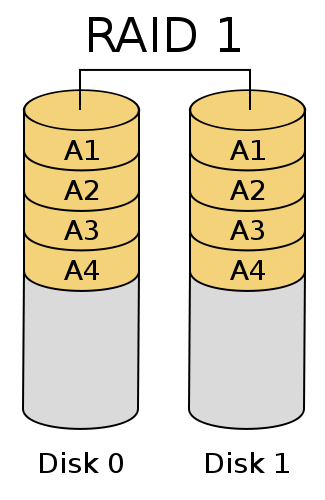
\includegraphics[width=\textwidth]{imagens/RAID_1}
			\label{fig:exemplo}
		\end{figure}
		
	\end{columns}
\end{frame}

\begin{frame}{RAID 5}
	\begin{columns}
		\column{0.5\textwidth}
		\begin{itemize}
			\item Esquema de paridade, pelo uso do bloco de paridade.
			\item A informação sobre paridade é distribuída entre todos os discos.
			\item Vantagens
			\begin{itemize}
				\item Tolerância a falhas.
				\item Leitura rápida.
			\end{itemize}
			\item Desvantagens
			\begin{itemize}
				\item Sistema complexo de controle dos discos.
			\end{itemize}
		\end{itemize}
		
		\column{0.5\textwidth}
		\begin{figure}
			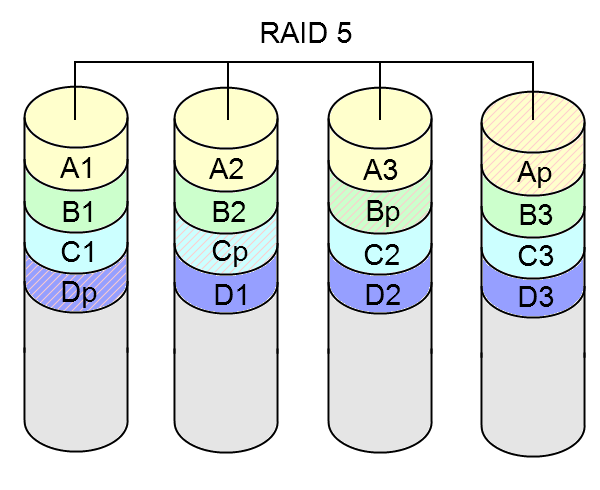
\includegraphics[width=\textwidth]{imagens/RAID_5}
			\label{fig:exemplo}
		\end{figure}
		
	\end{columns}
\end{frame}